\chapter{Attachments} \label{chap:attachments}

% ~~~~~~~~~~~~~~~~~~~~~~~~~~~~~~~~~~~~~~~~~~~~~~~~~~~~~~~~~~~~~~~~~~~~~~~~~~~~~~~~~~~~~~~~~~~~~~~~~~~~~~~~~~~
\section{Algorithms, Functions, and Procedures} \label{sec:attachments/algorithms-functions-procedures}


\begin{alg}{Function}{GranularResourceLoad}{$k$, $\Instance$, $\Schedule$, $PC$} \label{alg:granular-resource-load}
\State $L : \intinterval{1}{PC} \to \Nzero$
       \Comment Period load function
\For {$j \in \JobsOnResource{k}$}
    \State $i_l \gets \lfloor \jobstart{j} / \algGranularity \rfloor$,
           \Comment{First overlapping period}
    \State $i_h \gets \lfloor \jobend{j} / \algGranularity \rfloor$
           \Comment{Last overlapping period}
    \If {$i_l = i_h$}
        \Comment{If the job overlaps with a single period...}
        \State $L(i_l) \gets L(i_l) + \duration{j} \consumption{j}{k}$
    \Else
        \Comment{...the job overlaps with multiple periods}
        \State $L(i_l) \gets L(i_l) + (\algGranularity (i_l + 1) - \jobstart{j}) \cdot \consumption{j}{k}$
        \For {$i \in \intinterval{i_l+1}{i_h-1}$}
            \State $L(i) \gets L(i) + \algGranularity \cdot \consumption{j}{k}$
        \EndFor
        \State $L(i_h) \gets L(i_h) + (\jobend{j} - \algGranularity (i_h - 1)) \cdot c$
    \EndIf
\EndFor
\State \Return $L$
\end{alg}


\begin{alg}{Function}{IncreaseGranularPeriodCapacity}{$i$, $\capacityf{k}$, $\algGranularity$, $\algImprovement$} \label{alg:increase-granular-period-capacity}
\State $t_l \gets 1+ (i-1)\algGranularity$
       \Comment First time period covered
\State $t_h \gets i \algGranularity$
       \Comment Last time period covered
\For{$t \in \intinterval{t_l}{t_h}$}
    \State $\capacity{k}{t} \gets \capacity{k}{t} + \algImprovement$
\EndFor
\State \Return $\capacity{k}{t}$
\end{alg}


\begin{alg}{Function}{ReduceCapacityChanges}{$\Instance$, $\Schedule$, $\capacityf{1}^\text{orig}$, \dots, $\capacityf{m}^\text{orig}$} \label{alg:reduce-capacity-changes}
\State $\capacityf{1}^\prime, \dots, \capacityf{m}^\prime: \intinterval{1}{\horizon} \to \Nzero$
       \Comment Reduced capacity functions
\For {$k \in \Resources$}
    \State $L \gets $ \Call{ResourceLoad}{$k$, $\Instance$, $\Schedule$}
    \For {$t \in \intinterval{1}{\horizon}$}
        \State $\capacity{k}{t}^\prime \gets \max(\capacity{k}{t}^{\text{orig}}, L(t))$
    \EndFor
\EndFor
\State \Return $\capacityf{1}^\prime, \dots, \capacityf{m}^\prime$
\end{alg}


\begin{alg}{Function}{ResourceLoad}{$k$, $\Instance$, $\Schedule$} \label{alg:resource-load}
\State $L : \intinterval{1}{\horizon} \to \Nzero$
\For {$t \in \intinterval{1}{\horizon}$}
    \State $L(t) \gets \sum_{j \in \JobsOnResourceInTimePeriod{k}{t}} \consumption{j}{k}$
        \Comment $\JobsOnResourceInTimePeriod{k}{t}$ with respect to given schedule $\Schedule$
\EndFor
\State \Return $L$
\end{alg}


\todo{FindAdditionsAndMigrations}
\begin{alg}{Function}{FindAdditionsAndMigrations}{$\capacityf{k}$, $\Instance$, $\Schedule$} \label{alg:find-additions-and-migrations}
\State REQ $\gets$ set of all capacity addition requirements
\State 
\end{alg}


\begin{alg}{Function}{ModifyResourceCapacities}{$\Instance$, $\chi_1$, \dots, $\chi_c$} \label{alg:modify-resource-capacities}
\State $\capacityf{1}^*, \dots, \capacityf{m}^* \gets \capacityf{1}, \dots, \capacityf{m}$
    \Comment Copy the original capacity functions
\For {$(j, s, e) \in \{ \chi_1, \dots, \chi_c \}$}
    \For {$k \in \Resources : \consumption{j}{k} > 0 $}
        \For {$t \in \intinterval{s}{e-1}$}
            \State $\capacity{k}{t}^* \gets \capacity{k}{t}^* + \consumption{j}{k}$
        \EndFor
    \EndFor
\EndFor
\State \Return $\capacityf{1}^*, \ldots, \capacityf{m}^*$
\end{alg}

% ~~~~~~~~~~~~~~~~~~~~~~~~~~~~~~~~~~~~~~~~~~~~~~~~~~~~~~~~~~~~~~~~~~~~~~~~~~~~~~~~~~~~~~~~~~~~~~~~~~~~~~~~~~~
\section{Full instance plots} \label{sec:attachments/full-instance-plots}

\begin{figure}
    \centering
    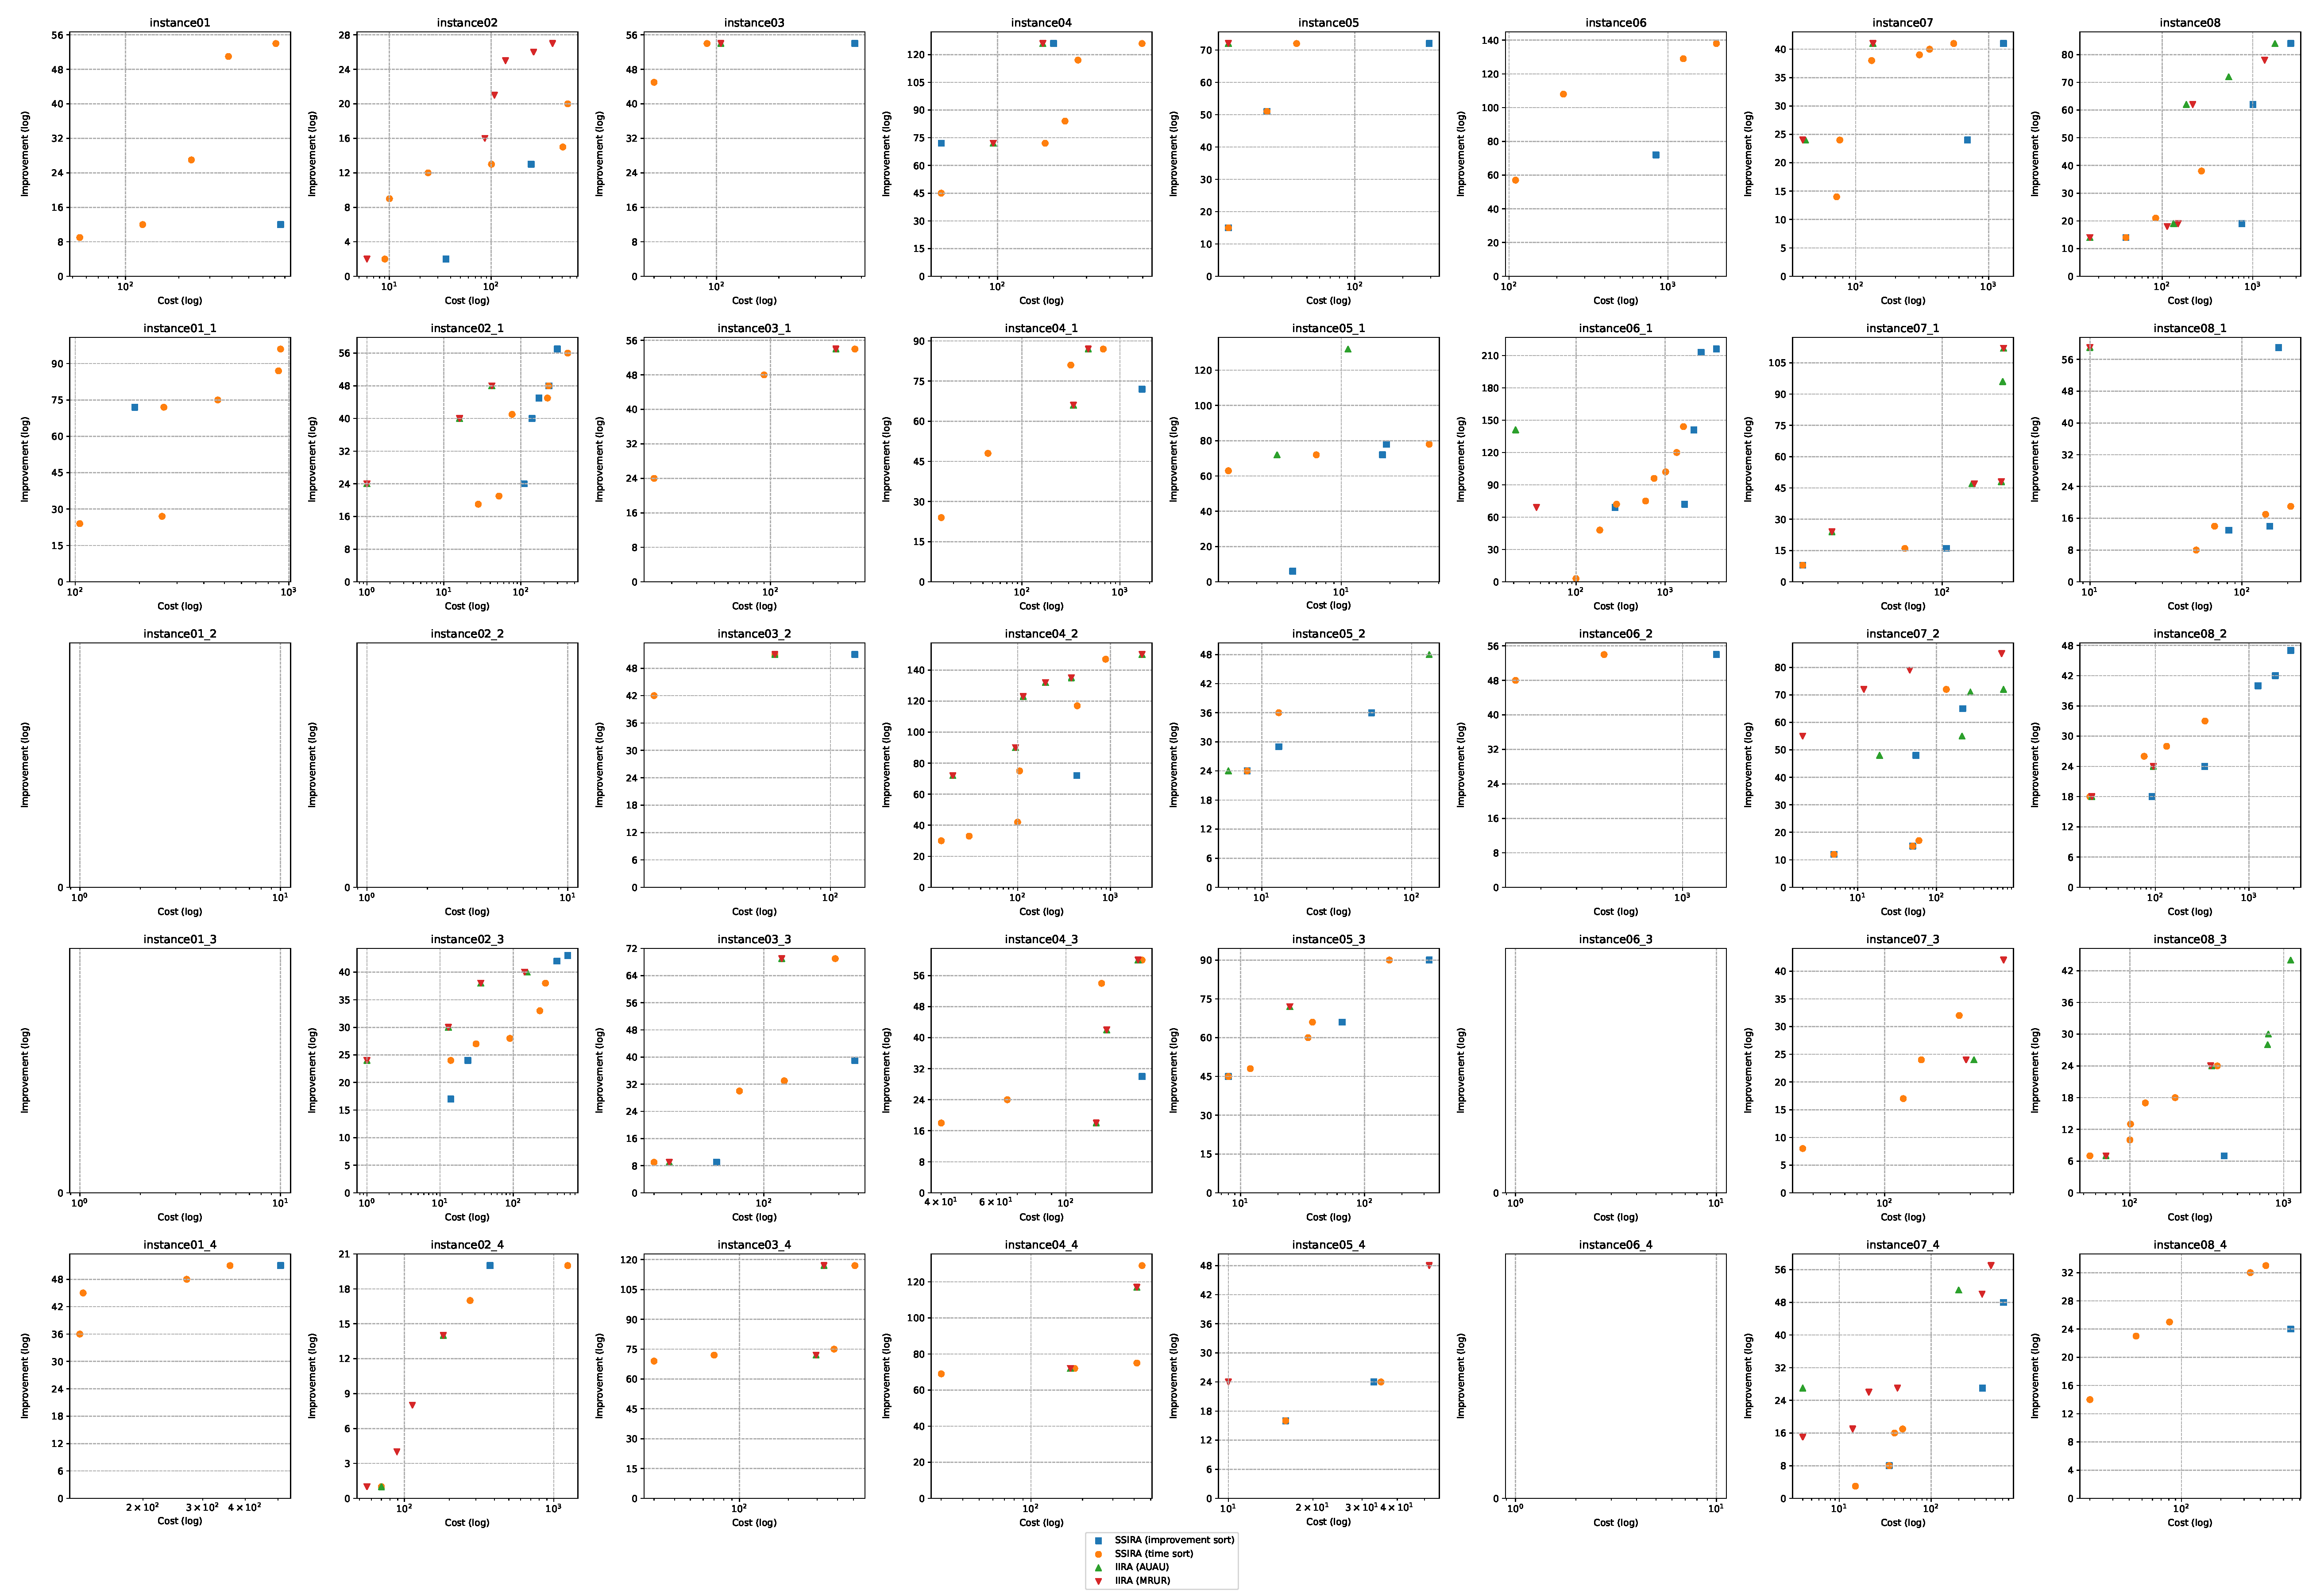
\includegraphics[angle=270, width=\textwidth]{img/exp_cost_improv.pdf}
    \caption{
        Capacity changes cost (x-axis) to achieved 
        improvement (y-axis) for every experiment instance.
        }
    \label{fig:exp-full/cost-improv}
\end{figure}

\begin{figure}
    \centering
    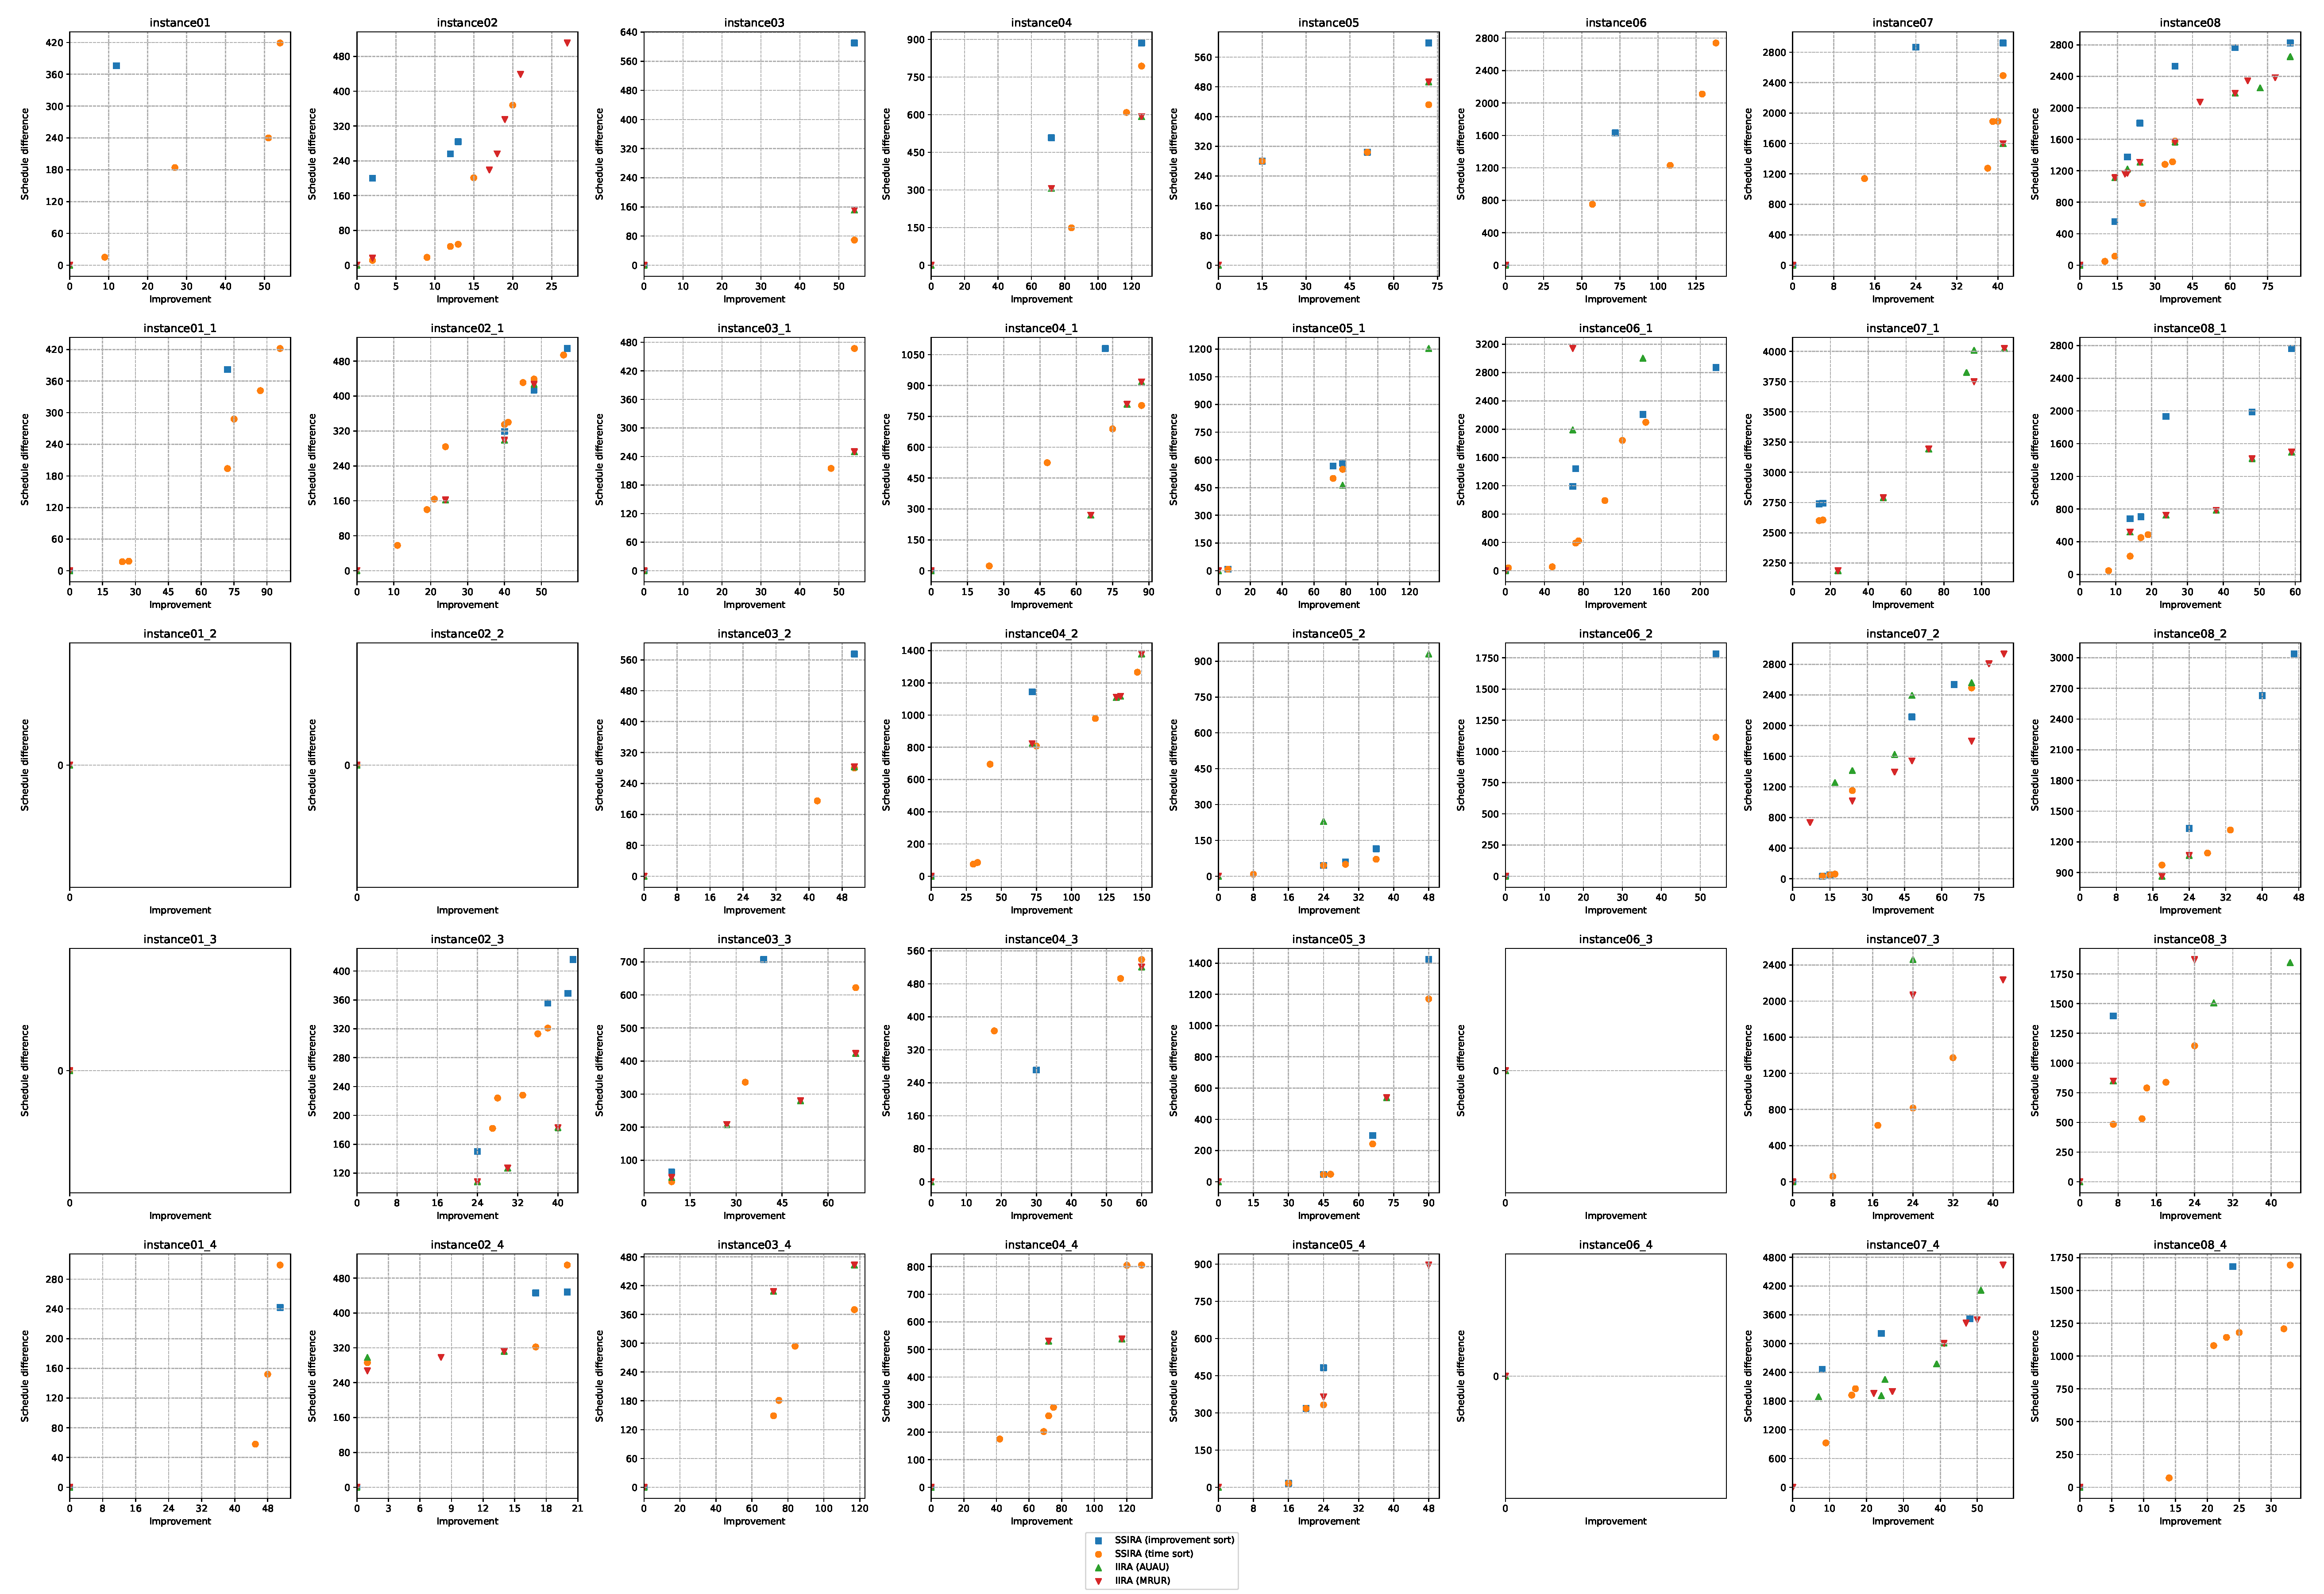
\includegraphics[angle=270,width=\textwidth]{img/exp_improv_diff.pdf}
    \caption{
        Achieved improvement (x-axis) to schedule
        difference (y-axis) for every experiment instance.
        }
    \label{fig:exp-full/improv-diff}
\end{figure}

\begin{figure}
    \centering
    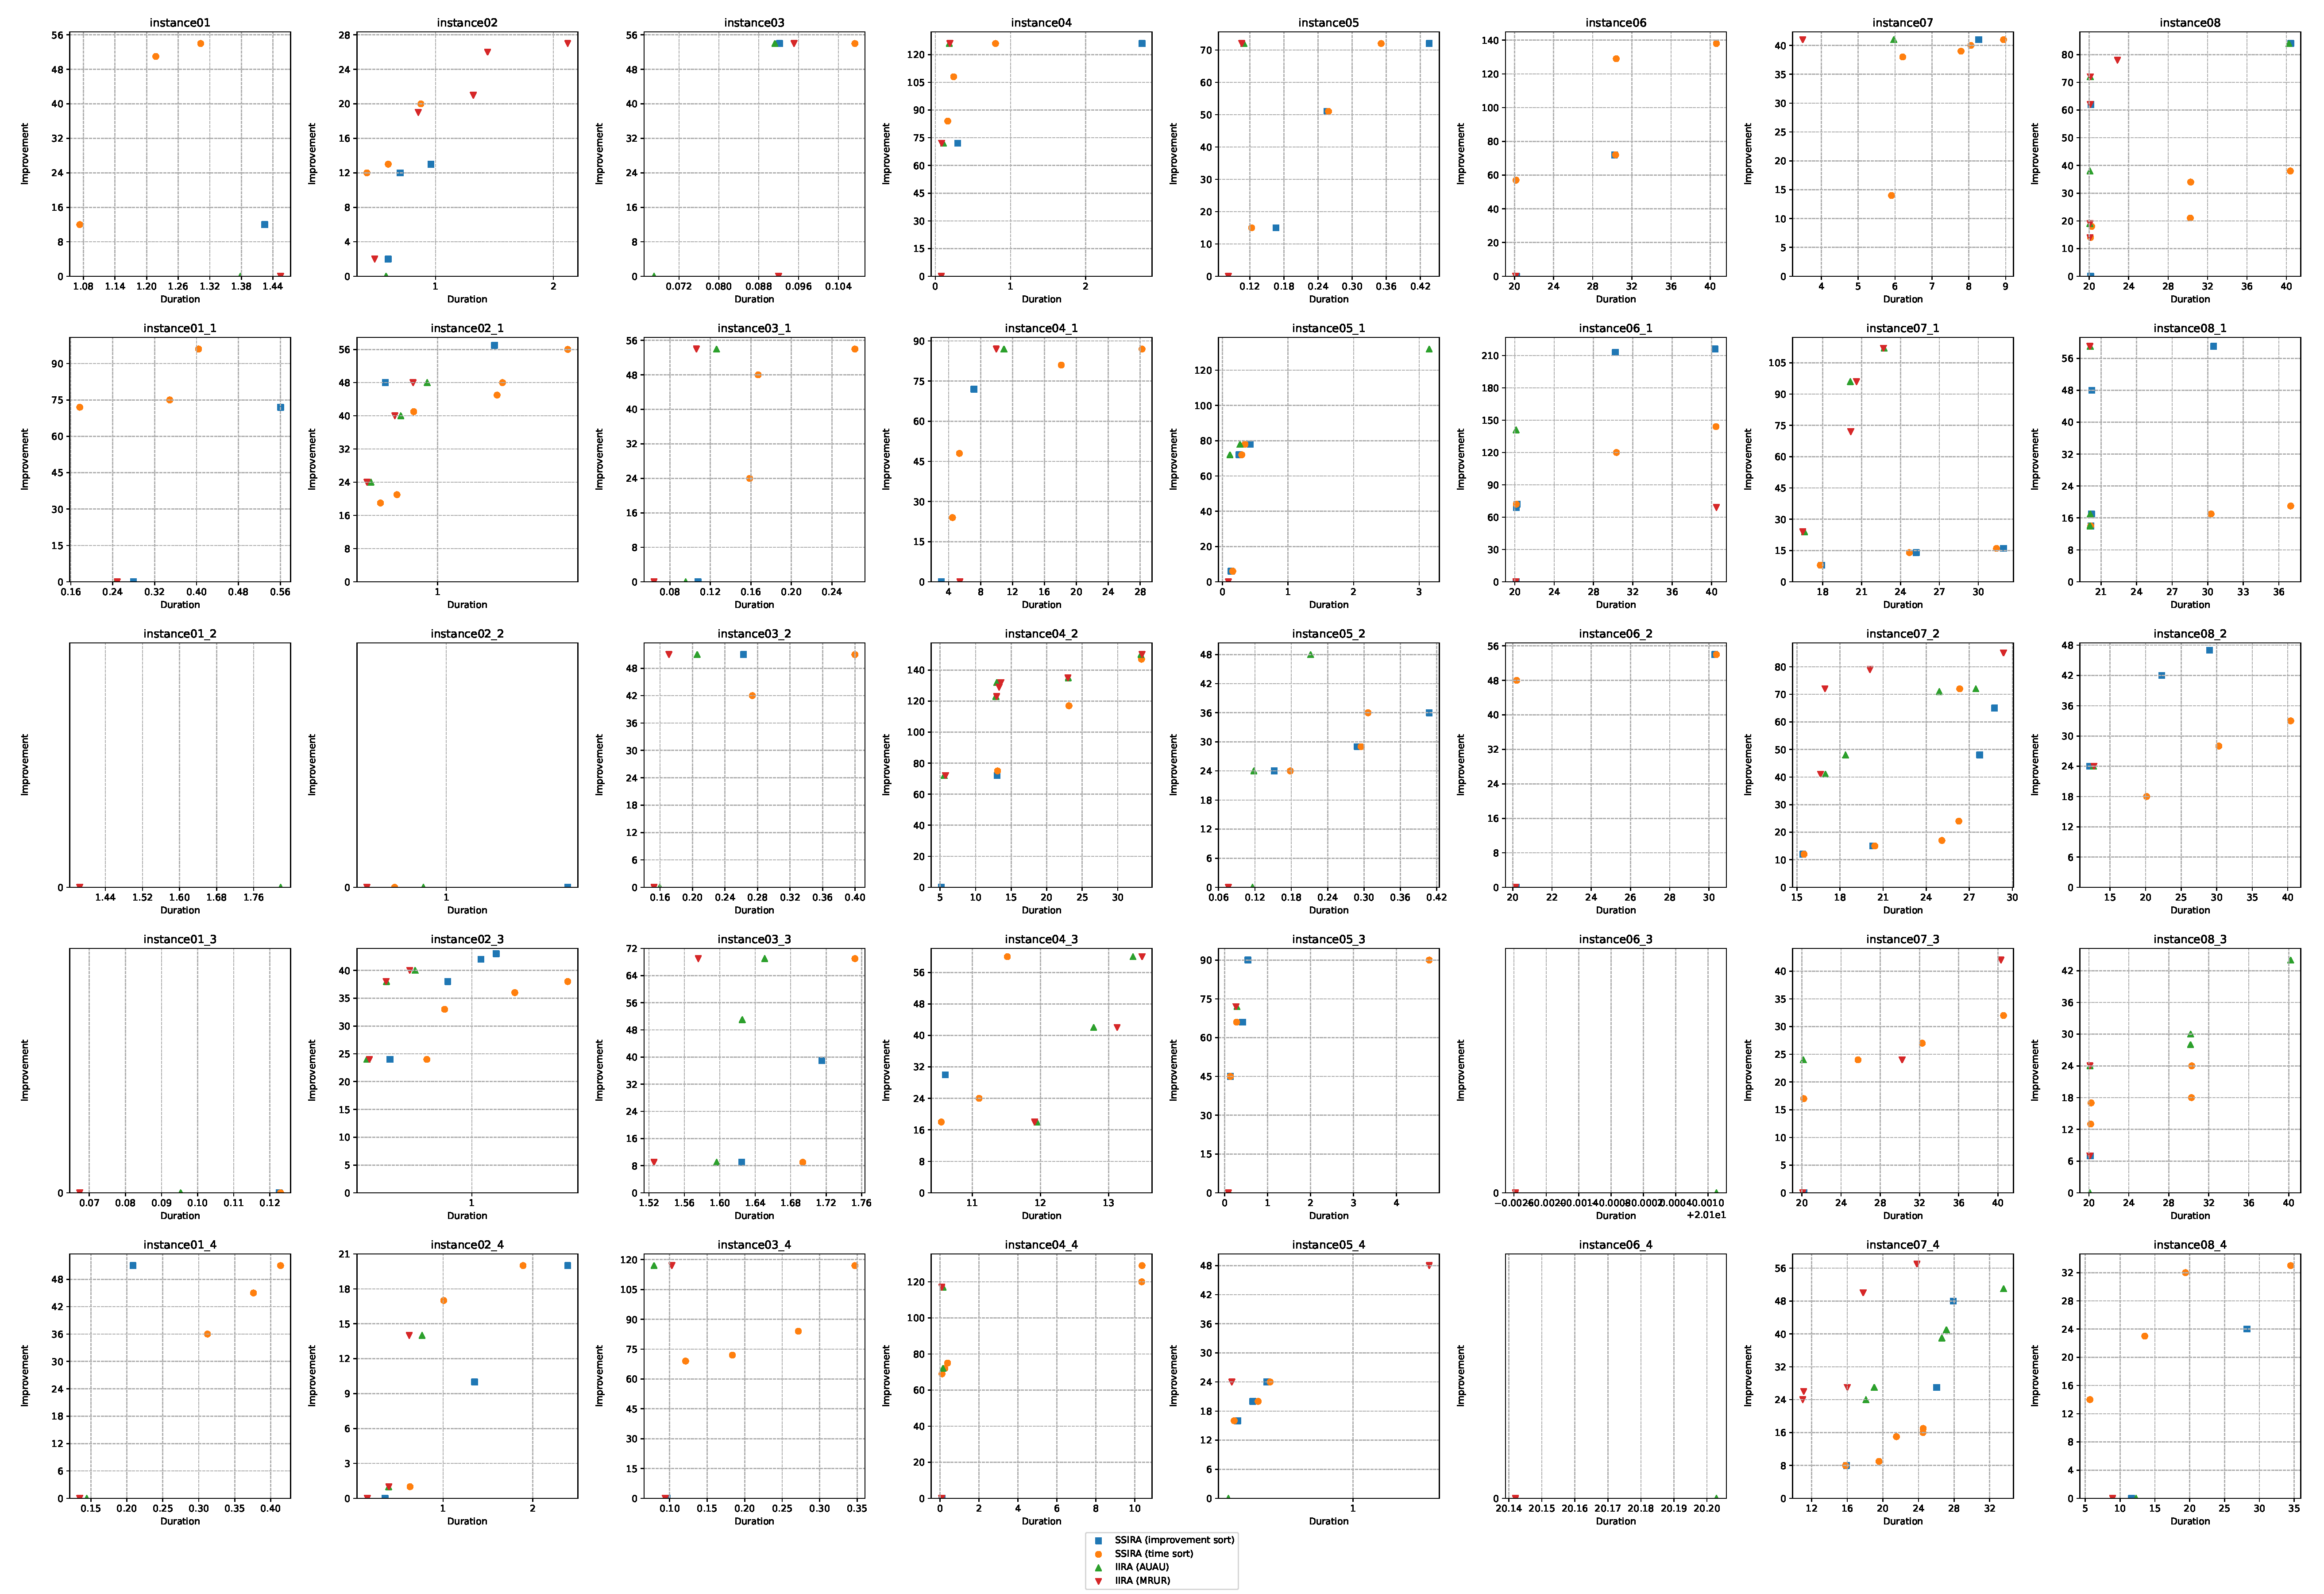
\includegraphics[angle=270,width=\textwidth]{img/exp_duration_improv.pdf}
    \caption{
        Evaluation duration (x-axis) to achieved
        improvement (y-axis) for every experiment instance.
        }
    \label{fig:exp-full/duration-improv}
\end{figure}

% ~~~~~~~~~~~~~~~~~~~~~~~~~~~~~~~~~~~~~~~~~~~~~~~~~~~~~~~~~~~~~~~~~~~~~~~~~~~~~~~~~~~~~~~~~~~~~~~~~~~~~~~~~~~
\section{Documentation} \label{sec:attachments/documentation}

\begin{small}
\begin{verbatim}
usage: experiments.py [--aggregate] [--scale] [--save_plots]
                      [--addition ADDITION] [--migration MIGRATION]
                                                                                                               
options:                                                                                                       
  --aggregate            Determines whether to aggregate
                         instances by type                                      
  --scale                Determines whether to scale
                         evaluations KPIs                                           
  --save_plots           Determines whether to save plots to files                                              
  --addition ADDITION    Cost of capacity addition                                                              
  --migration MIGRATION  Cost of capacity migration
\end{verbatim}
\end{small}


